\chapterimage{chap32.jpg}
\chapter{June}
\section{Week \Rmnum{1}}
\hl{\textbf{\textit{June 1}}}

1.$\lim\limits_{x\rightarrow 0}\dfrac{\tan(\sin x)-x}{\arctan x-\arcsin x}$
\myspace{1}
\begin{solution}
	
	原极限等价于: 
	$$\lim\limits_{x\rightarrow 0}\dfrac{\tan(\sin x)-\sin x}{\arctan x-\arcsin x}+\lim\limits_{x\rightarrow 0}\dfrac{\sin x-x}{\arctan x-\arcsin x}$$
	$$I_{1}=\lim\limits_{x\rightarrow 0}\dfrac{\frac{1}{3}\sin^3 x}{-\frac{1}{2}x^3}=-\frac{2}{3}$$
	$$I_{2}=\lim\limits_{x\rightarrow 0}\dfrac{-\frac{1}{6} x^3}{-\frac{1}{2}x^3}=\frac{1}{3}$$
	$$I=I_{1}+I_{2}=-\frac{1}{3}$$
\end{solution}
\myspace{1}

2. 设$\{x_{n}\},\{y_{n}\}$满足$x_{1}=y_{1}=\dfrac{1}{2}$,$x_{n+1}=\sin x_{n}$,$y_{n+1}=y_{n}^2$,判断$x_{n}$和$y_{n}$的阶数
\begin{itemize}
	\item A.$\{x_{n}\}\text{比}\{y_{n}\}\text{高阶}$
	\item \hl{B}.$\{y_{n}\}\text{比}\{x_{n}\}\text{高阶}$
	\item C.$\{x_{n}\}\text{和}\{y_{n}\}\text{等价}$
	\item D.$\{x_{n}\}\text{和}\{y_{n}\}\text{同阶不等价}$
\end{itemize}
\myspace{1}
\begin{solution}
	
	我们用数学归纳法来证明: 
	$$0<y_{n}\leq x_{n}\leq \frac{1}{2}$$
	
	(1).当$n=1$时,上式显然成立
	
	(2).假设当$n=k$时上式成立
	
	(3).当$n=k+1$时: 
	$$x_{k+1}=\sin x_{k}<\sin \frac{\pi}{6}=\frac{1}{2}$$
	$$y_{k+1}=y_{k}^2<\frac{1}{2}$$
	$$\text{我们有}x_{k}\geq \sin x_{k}\geq x_{k}^2\geq y_{k}^2\Rightarrow x_{k+1}\geq y_{k+1}$$
	
	我们得到: 
	$$\dfrac{y_{n+1}}{x_{n+1}}<\dfrac{\frac{1}{2}y_{n}}{\frac{2}{\pi}x_{n}}=\dfrac{\pi}{4}\dfrac{y_{n}}{x_{n}}<(\dfrac{\pi}{4})^n$$
	
	两边取极限,由夹逼定理可以得到: 
	$$\lim\limits_{n\rightarrow +\infty}\frac{y_{n}}{x_{n}}=0$$
\end{solution}
\myspace{1}

\hl{\textbf{\textit{June 2}}}

1. $f(x)$可微,且$x=\int_{0}^{x}f(t)dt+\int_{0}^{x}tf(t-x)dt$,求$f(x)$
\myspace{1}
\begin{solution}
	
	我们对方程后面部分$\int_{0}^{x}tf(t-x)dt$进行换元,得到: 
	$$\int_{0}^{x}tf(t-x)dt=x\in_{-x}^{0}f(-t)dt+\int_{-x}^{0}tf(t)dt$$
	
	我们对方程两边对$x$求导,得到: 
	$$f(x)+\int_{0}^{x}f(-t)dt=1\Rightarrow f'(x)+f(-x)=0\Leftrightarrow f'(-x)+f(x)=0$$
	
	我们继续对$x$求导得到: 
	$$f''(x)-f'(-x)=0\Rightarrow f''(x)+f(x)=0$$
	
	$$f(x)=c_{1}\sin x+c_{2}\cos x,f(0)=1,f'(0)=-1\Rightarrow c_{1}=-1.c_{2}=1$$
	
	$$f(x)=\cos x-\sin x$$
\end{solution}
\myspace{1}

\hl{\textbf{\textit{June 3}}}

1. $\lim\limits_{x\rightarrow 0}\dfrac{\sqrt[4]{1-\sqrt[3]{1-\sqrt{1-x}}}-1}{(1+x)^{\frac{1}{\sqrt[3]{x^2}}}-1}$
\myspace{1}
\begin{solution}
	
	原极限等价于: 
	$$I=-\frac{1}{4}\lim\limits_{x\rightarrow 0}\dfrac{\sqrt[3]{1-\sqrt{1-x}}}{x^{-\frac{2}{3}}\ln(1+x)}=-\frac{1}{4}\lim\limits_{x\rightarrow 0}\dfrac{\sqrt[3]{x}}{\sqrt[3]{x}\sqrt[3]{1+\sqrt{1-x}}}=-\frac{1}{4\sqrt[3]{2}}$$
\end{solution}
\myspace{1}

2. $y''+ay'=f(x),a>0$,$f(+\infty)=b$,求$\lim\limits_{x\rightarrow +\infty}y''(x)$
\myspace{1}
\begin{solution}
	
	我们由$y''+ay'=f(x),a>0$,利用一阶线性微分方程通解公式得到: 
	$$y'=e^{-ax}\left(\int_{0}^{x}e^{at}f(t)dt+C \right) $$
	
	我们得到: 
	$$\lim\limits_{x\rightarrow +\infty}y'=\lim\limits_{x\rightarrow +\infty}\dfrac{\left(\int_{0}^{x}e^{at}f(t)dt+C \right)}{e^{ax}}=\lim\limits_{x\rightarrow +\infty}\dfrac{e^{ax}f(x)}{ae^{x-1}}=\dfrac{b}{a}$$
	
	我们又有: $y''+ay'=f(x)$
	
	$$\lim\limits_{x\rightarrow +\infty}y''=\lim\limits_{x\rightarrow +\infty}[f(x)-ay']=0$$
\end{solution}
\myspace{1}

\hl{\textbf{\textit{June 4}}}

1. $\lim\limits_{x\rightarrow 0}\dfrac{(3+\sin x^2)^{x}-3^{\sin x}}{x^3}$
\myspace{1}
\begin{solution}
	
	我们令$f(x)=e^x$,由拉格朗日中值定理得到: 
	$$\exists \xi\in(x\ln 3,x\ln(3+x^2)),\ s.t. e^{x\ln(3+x^2)}-e^{\sin x\ln 3}=e^{\xi}[x\ln(3+\sin x^2)-\sin x\ln 3]$$
	
	由夹逼定理得到: 
	$$\lim\limits_{x\rightarrow 0 }x\ln 3=\lim\limits_{x\rightarrow 0 }x\ln(3+x^2)=0\Rightarrow \lim\limits_{x\rightarrow 0 }e^{\xi}=1$$
	
	原极限等价于: 
	\begin{eqnarray*}
		I&=&\lim\limits_{x\rightarrow 0}e^{\xi}\lim\limits_{x\rightarrow 0}\dfrac{[x\ln(3+\sin x^2)-x\ln 3+x\ln 3-\sin x\ln 3]}{x^3}\\
		&=&\lim\limits_{x\rightarrow 0}\dfrac{[x\ln(3+\sin x^2)-x\ln 3]}{x^3}+\lim\limits_{x\rightarrow 0}\dfrac{x\ln 3-\sin x\ln 3}{x^3}\\
		&=&\dfrac{2+\ln 3}{6}
	\end{eqnarray*}
	
	综上所述,原极限$I=\dfrac{2+\ln 3}{6}$
\end{solution}
\myspace{1}

2. $\sum\limits_{n=1}^{+\infty}n(n+1)x^n$
\myspace{1}
\begin{solution}
	
	幂级数的收敛域: 
	$$\rho=\lim\limits_{n\rightarrow+\infty}\dfrac{(n+1)(n+2)}{n(n+1)}=1\Rightarrow R=1,\text{幂级数收敛域为}(-1,1)$$
	原幂级数可化为: 
	\begin{eqnarray*}
		S(x)&=&x\sum\limits_{n=1}^{+\infty}n(n+1)x^{n-1}\\&=&x\sum\limits_{n=1}^{+\infty}(x^{n+1})''\\&=&x\left( \sum\limits_{n=1}^{+\infty}x^{n+1}\right) ''\\
		&=&x\left( \dfrac{x^2}{1-x}\right) ''\\
		&=&\dfrac{-2x}{(x-1)^3},x\in(-1,1)
	\end{eqnarray*}
\end{solution}
\myspace{1}

\hl{\textbf{\textit{June 5}}}

1. 设$f(x)$在$[0,2\pi]$连续可导,$f'(x)\geq 0$,证明: 
$$\left| \int_{0}^{2\pi}f(x)\sin nxdx\right|\leq \dfrac{2}{n}[f(2\pi)-f(0)] $$
\myspace{1}
\begin{solution}
	
	由分部积分法: 
	\begin{eqnarray*}
		\left| \int_{0}^{2\pi}f(x)\sin nxdx\right|&=&\dfrac{1}{n}\left| \int_{0}^{2\pi}f(x)d\cos nx\right|\\
		&=&\dfrac{1}{n}\left| f(x)\cos nx|_{0}^{2\pi}-\int_{0}^{2\pi}f'(x)\cos nxdx\right|\\
		&\leq &\dfrac{1}{n}[f(2\pi)-f(0)]+|\int_{0}^{2\pi}f'(x)\cos nxdx|\\
		&=&\dfrac{1}{n}[f(2\pi)-f(0)]+|\int_{0}^{2\pi}f'(x)dx|\\
		&=&\dfrac{2}{n}[f(2\pi)-f(0)]
	\end{eqnarray*}
\end{solution}
\myspace{1}

2. 证明$\left| \int_{x}^{x+1}\sin t^2dt\right| \leq \dfrac{1}{x}$
\myspace{1}
\begin{solution}
	
	分部积分: 
	\begin{eqnarray*}
		I&=&\frac{1}{2}\left| \int_{x}^{x+1}\frac{1}{t}d\cos t^2\right|\\
		&=&\frac{1}{2}\left| \frac{1}{t}\cos t^2|_{x}^{x+1}+ \int_{x}^{x+1}\frac{1}{t^2}\cos t^2dt\right|\\
		&\leq&\frac{1}{2}[\left| \frac{1}{t}\cos t^2|_{x}^{x+1}\right|+\left|  \int_{x}^{x+1}\frac{1}{t^2}dt\right|]\\
		&=&\frac{1}{2}[\frac{\cos x^2}{x}-\frac{\cos(x+1)^2}{x+1}+\frac{1}{x}-\frac{1}{x+1}]\\
		&\leq&\frac{1}{x}
	\end{eqnarray*}
\end{solution}
\myspace{1}

\hl{\textbf{\textit{June 6}}}

1. $\lim\limits_{x\rightarrow 1}\dfrac{x-x^{x}}{1-x+\ln x}$
\myspace{1}
\begin{solution}
	
	原极限可以写作: 
	\begin{eqnarray*}
		I&=&\lim\limits_{x\rightarrow 1}\dfrac{x-e^{x\ln x}}{1-x+\ln(1+x-1)}(\text{泰勒展开})\\
		&=&\lim\limits_{x\rightarrow 1}\dfrac{x-(1+x(x-1))}{1-x+(x-1)-\frac{1}{2}(x-1)^2}\\
		&=&2
	\end{eqnarray*}
\end{solution}
\myspace{1}

2. $\sum\limits_{n=1}^{+\infty}\dfrac{n}{(n+1)!}$
\myspace{1}
\begin{solution}
	
	原级数等价于: 
	\begin{eqnarray*}
		S&=&\lim\limits_{n\rightarrow+\infty}u_{n}\\
		&=&\lim\limits_{n\rightarrow+\infty}(\dfrac{1}{n!}-\dfrac{1}{(n+1)!})\\
		&=&\lim\limits_{n\rightarrow+\infty}(1-\dfrac{1}{(n+1)!})\\
		&=&1	
	\end{eqnarray*}
\end{solution}
\myspace{1}

\hl{\textbf{\textit{June 7}}}

1. 设函数$u=f(x,y,x)$有连续偏导数,且$z=z(x,y)$由方程$xe^x-ye^y=ze^z$所确定,求$du$
\myspace{1}
\begin{solution}
	
	我们得到关于$x,y,z$的方程$F(x,y,z)$,利用隐函数导数公式: 
	$$\dfrac{\partial z}{\partial x}=-\dfrac{F_{x}}{F_{z}}=\dfrac{(x+1)e^x}{(z+1)e^z},\ \dfrac{\partial z}{\partial y}=-\dfrac{F_{y}}{F_{z}}=-\dfrac{(y+1)e^y}{(z+1)e^z}$$
	
	我们得到: 
	$$\left\lbrace 
	\begin{array}{l}
		\dfrac{\partial u}{\partial x}=f_{1}+f_{3}\dfrac{\partial z}{\partial x}=f_{1}+f_{3}\dfrac{(x+1)e^x}{(z+1)e^z}\\
		\dfrac{\partial u}{\partial y}=f_{2}+f_{3}\dfrac{\partial z}{\partial y}=f_{1}-f_{3}\dfrac{(y+1)e^y}{(z+1)e^z}
	\end{array}
	\right. $$
	
	$$du=(f_{1}+f_{3}\dfrac{(x+1)e^x}{(z+1)e^z})dx+(f_{1}-f_{3}\dfrac{(y+1)e^y}{(z+1)e^z})dy$$
\end{solution}
\myspace{1}

2. 设$u=f(x,y,z)$,$\varphi(x^2,e^y,z)=0$,$y=\sin x$确定了函数$u(x)$,其中$f,\varphi$具有一阶偏导数,且$\dfrac{\partial \varphi}{\partial z}\neq 0$,求$\dfrac{du}{dx}$
\myspace{1}
\begin{solution}
	
	复合函数偏导数: 
	$$\dfrac{du}{dx}=f_{1}+f_{2}\dfrac{dy}{dx}+f_{3}(\dfrac{\partial z}{\partial x}+\dfrac{\partial z}{\partial y}\dfrac{dy}{dx})$$
	
	$$\dfrac{dy}{dx}=\cos x,\ \dfrac{\partial z}{\partial x}=-\dfrac{2x\varphi_{1}}{\varphi_{3}},\ \dfrac{\partial z}{\partial y}=-\dfrac{e^y\varphi_{2}}{\varphi_{3}}$$
	
	我们最终得到$\dfrac{du}{dx}$: 
	$$\dfrac{du}{dx}=f_{1}+f_{2}\cos x-f_{3}\dfrac{2x\varphi_{1}+e^{\sin x}\cos x \varphi_{2}}{\varphi_{3}}$$
\end{solution}
\myspace{1}

\section{Week \Rmnum{2}}
\hl{\textbf{\textit{June 8}}}

1. $$\lim\limits_{t\rightarrow 0^{+}}\lim\limits_{x\rightarrow+\infty}\dfrac{\int_{0}^{\sqrt{t}}dx\int_{x^2}^{t}\sin y^2dy}{\left[\left( \frac{2}{\pi}\arctan \frac{x}{t^2}\right)^{x}-1\right]\int_{0}^{t}(e^{\sqrt{u}}-1)du }$$
\myspace{1}
\begin{solution}
	
	原极限可以化为: 
	\begin{eqnarray*}
		I&=&\lim\limits_{t\rightarrow 0^{+}}\lim\limits_{x\rightarrow+\infty}\dfrac{\int_{0}^{t}dy\int_{0}^{\sqrt{t}}\sin y^2dy}{[e^{x\ln(\frac{2}{\pi}\arctan \frac{x}{t^2})}-1]\int_{0}^{t}(e^{\sqrt{u}}-1)du}\\
		&=&\lim\limits_{t\rightarrow 0^{+}}\lim\limits_{x\rightarrow+\infty}\dfrac{\int_{0}^{t}\sqrt{y}\sin y^2dy}{\int_{0}^{t}(e^{\sqrt{u}}-1)du[e^{-\frac{x\pi}{2}\arctan\frac{t^2}{x}}-1]}\\
		&=&\lim\limits_{t\rightarrow 0^{+}}\dfrac{\int_{0}^{t}\sqrt{y}\sin y^2dy}{[e^{-\frac{2t^2}{\pi}}-1]\int_{0}^{t}(e^{\sqrt{u}}-1)du}\\
		&=&\lim\limits_{t\rightarrow 0^{+}}\dfrac{\frac{2}{7}t^{\frac{7}{2}}}{-\frac{4}{3\pi}t^{\frac{7}{2}}}\\
		&=&-\dfrac{3\pi}{14}
	\end{eqnarray*}
\end{solution}
\myspace{1}

2. 求极限$\lim\limits_{x\rightarrow 0}\dfrac{(1+x)^{\frac{2}{x}}-e^2[1-\ln(e^x+\sin x)]}{x}$
\myspace{1}
\begin{solution}
	
	原极限可化为: 
	\begin{eqnarray*}
		I&=&\lim\limits_{x\rightarrow 0}\dfrac{e^2[e^{\frac{2\ln(1+x)}{x}-2}+\ln(e^x+\sin x)-1]}{x}\\
		I_{1}&=&\lim\limits_{x\rightarrow 0}\dfrac{\frac{2\ln(1+x)}{x}-2}{x}=\lim\limits_{x\rightarrow 0}\dfrac{2\ln(1+x)-2x}{x^2}=-1\\
		I_{2}&=&\lim\limits_{x\rightarrow 0}\dfrac{\ln(1+e^x+\sin x-1)}{x}=\lim\limits_{x\rightarrow 0}\dfrac{e^x+\sin x-1}{x}=2\\
		I&=&e^2(I_{1}+I_{2})=e^2
	\end{eqnarray*}
\end{solution}
\myspace{1}

\hl{\textbf{\textit{June 9}}}

1. $f(x)$二阶可导,$f(a)=f'(a)=f''(a)=f(b)=0$,证明: $\exists \xi\in(a,b),\ s.t. (\xi-a)^2f''(\xi)-2f(\xi)=0$
\myspace{1}
\begin{solution}
	
	我们令$g(x)=(x-a)^2,g'(x)=2(x-a),g''(x)=2$
	
	原式等价于: $\exists \xi\in(a,b),\ s.t. g(\xi)f''(\xi)-g''(\xi)f(\xi)=0$
	
	我们构造辅助函数: $F(x)=\dfrac{f(x)}{g(x)}$
	$$F'(x)=\dfrac{f'(x)g(x)-g'(x)f(x)}{g^2(x)}$$
	
	我们对分子继续求导: 
	$$(f'(x)g(x)-g'(x)f(x))'=f''(x)g(x)+f'(x)g'(x)-g''(x)f(x)-g'(x)f'(x)=f''(x)g(x)-g''(x)f(x)$$
	
	此时$F(x)=\dfrac{f(x)}{(x-a)^2}$,$\lim\limits_{x\rightarrow a}F(x)=0$,我们构造: 
	$$F(x)=\left\lbrace 
	\begin{array}{l}
		\dfrac{f(x)}{(x-a)^2},x\in(a,b]\\
		0,x=a
	\end{array}
	\right. $$
	
	$F(x)$在区间$[a,b]$上连续,且$F(a)=F(b)=0$
	
	我们在区间$(a,b)$上对$F(x)$使用罗尔定理得到: 
	$$\exists c\in(a,b),\ s.t. F'(c)=0\Rightarrow (c-a)^2f'(c)-2(c-a)f(c)=0$$
	
	对于函数$H(x)=(x-a)^2f'(x)-2(x-a)f(x)$,我们有: $H(a)=H(c)=0$
	
	我们对$H(x)$在区间$(a,c)$上使用罗尔定理得到: 
	$$\exists\xi\in(a,c),\ s.t.H'(\xi)=0\Rightarrow  (\xi-a)^2f''(\xi)-2f(\xi)=0$$
	
\end{solution}
\myspace{1}

2. 求极限$\lim\limits_{x\rightarrow 0}\dfrac{(1+x)^{\frac{1}{x}}-(1+2x)^{\frac{1}{2x}}}{\sin x}$
\myspace{1}
\begin{solution}
	
	由拉格朗日中值定理: 
	$$e^{\frac{1}{x}\ln(1+x)}-e^{\frac{1}{2x}\ln(1+2x)}=e^{\xi}(\frac{1}{x}\ln(1+x)-\frac{1}{2x}\ln(1+2x)),\xi\in(\frac{1}{x}\ln(1+x),\frac{1}{2x}\ln(1+2x))$$
	
	原极限可化为: 
	\begin{eqnarray*}
		I&=&\lim\limits_{x\rightarrow 0}\dfrac{e^{\xi}[\frac{1}{x}\ln(1+x)-\frac{1}{2x}\ln(1+2x)]}{x}\\
		&=&\lim\limits_{x\rightarrow 0}e^{\xi}\dfrac{2\ln(1+x)-\ln(1+2x)}{2x^2}\\
		&=&\lim\limits_{x\rightarrow 0}e^{\xi}\dfrac{1}{2(1+x)(1+2x)}=\frac{e}{2}
	\end{eqnarray*}
\end{solution}
\myspace{1}

\hl{\textbf{\textit{June 10}}}

1. 设函数$f(x)$在区间$[0,2]$上具有连续导数,$f(0)=f(2)=0$,$M=max_{x\in[0,2]}\{|f(x)|\}$,证明: 

(1).$\exists\xi\in(0,2),\ s.t. |f'(\xi)|\geq M$

(2).若对任意的$x\in(0,2)$,$|f'(x)|\leq M$,则$M=0$
\myspace{1}
\begin{solution}
	
	(1). 我们不妨假设$|f(c)|=M$
	\begin{itemize}
		\item 当$c=0\text{或者}c=2$,我们得到: $f(x)\equiv 0$,我们得到: $M=0$,$\exists\xi\in(0,2),\ s.t. |f'(\xi)|\geq M$
		\item 当$c\in(0,2)$,$|f(c)|=M$,我们由拉格朗日中值定理得到: 
		$$\left\lbrace
		\begin{array}{l}
			f(c)-f(0)=cf'(\xi_{1}),\ \xi_{1}\in(0,c)\\
			f(2)-f(c)=(2-c)f'(\xi_{2}),\ \xi_{2}\in(c,2)
		\end{array}
		\right. \Rightarrow \left\lbrace
		\begin{array}{l}
			|f'(\xi_{1})|=\dfrac{M}{c},\ \xi_{1}\in(0,c)\\
			|f'(\xi_{2})|=\dfrac{M}{2-c},\ \xi_{2}\in(c,2)
		\end{array}
		\right. $$
		
		当$c\in(0,1],|f'(\xi_{1})|\geq M$;\ 当$c\in(1,2),|f'(\xi_{2})|\geq M$.
	\end{itemize}
	\myspace{1}
	
	(2).我们不妨假设$M>0$,$|f(d)|=M$,$f(0)=f(2)=0\Rightarrow \exists \eta\in(0,2),\ s.t. f'(\eta)=0$
	
	我们得到: 
	$$\left\lbrace
	\begin{array}{l}
		|f(d)-f(0)|=|\int_{0}^{d}f'(x)dx|\leq \int_{0}^{c}|f'(x)|dx\leq Md\\
		|f(2)-f(d)|=|\int_{d}^{2}f(x)dx|\leq \int_{d}^{2}|f(x)|dx\leq M(2-d)
	\end{array}
	\right.$$

	我们化简:
	$$\left\lbrace
	\begin{array}{l}
		M\leq Md\\
		M\leq M(2-d)
	\end{array}
	\right.  
	\Rightarrow 
	M(1-d)=0$$
	
	当$M=0$时,$f(x)\equiv 0$
	
	当$M\neq 0$,则$d=1$,$M=\left\lbrace
	\begin{array}{l}
		|f(1)-f(0)|\leq \int_{0}^{1}|f'(x)|dx\leq M\\
		|f(2)-f(1)|\leq \int_{1}^{2}|f'(x)|dx\leq M
	\end{array}
	\right. $	
	
	此时当且仅当$|f'(x)|\equiv M$时等号成立,如果$M\neq 0$,$f(2)\neq 0$,矛盾
	
	综上所述,$M=0$
\end{solution}
\myspace{1}

2. 求极限$\lim\limits_{x\rightarrow 0}\dfrac{1+\frac{x^2}{2}-\sqrt{1+x^2}}{(\cos x-e^{x^2})\sin x^2}$
\myspace{1}
\begin{solution}
	
	泰勒展开: 
	
	原极限可化为: 
	\begin{eqnarray*}
		I=\lim\limits_{x\rightarrow 0}\dfrac{1+\frac{x^2}{2}-(1+\frac{x^2}{2}+\frac{\frac{1}{2}(\frac{1}{2}-1)}{2}x^4)}{x^2(1-\frac{x^2}{2}-1-x^2)}=-\dfrac{1}{12}
	\end{eqnarray*}
\end{solution}
\myspace{1}

\hl{\textbf{\textit{June 11}}}

1. 证明方程$x^n+x^{n-1}+\cdots+x=1(n\geq 2)$在$(\frac{1}{2},1)$内有且仅有一个实数根,我们将这个实数根记作$x_{n}$,求$\lim\limits_{n\rightarrow+\infty}x_{n}$
\myspace{1}
\begin{solution}
	
	设函数$f(x)=x+x^2+\cdots+x^n-1$,我们有: $f'(x)=1+2x+3x^2+\cdots+nx^{n-1}>0\Rightarrow f(x)\text{在}(\frac{1}{2},1)\text{单调递增}$
	
	$$f(\frac{1}{2})=-\frac{1}{2^n}<0, f(1)=n-1>0$$
	
	根据零点定理,我们得到$f(x)$在区间$(\frac{1}{2},1)$内有且仅有一个零点.
	
	我们可以得到$\dfrac{1}{2}<x_{n}<1$
	
	我们知道: $f(x)$单调递增,当$x=x_{n}$时,我们有: 
	$$x_{n}+x_{n}^2+\cdots+x_{n}^n-1=0$$
	
	假设$x_{n+1}\geq x_{n}$,我们得到: 
	$$x_{n+1}+x_{n+1}^2+\cdots+x_{n+1}^n+x_{n+1}^{n+1}-1>x_{n}+x_{n}^2+\cdots+x_{n}^n-1=0$$
	
	我们要求: 
	$$x_{n+1}+x_{n+1}^2+\cdots+x_{n+1}^{n+1}-1=0\Rightarrow x_{n}>x_{n+1}$$
	
	$\{x_{n}\}$单调递减且有下界,$\{x_{n}\}$极限一定存在,我们不妨设$\lim\limits_{n\rightarrow +\infty}x_{n}=A$,我们有: 
	$$\dfrac{A}{1-A}=1\Rightarrow A=\dfrac{1}{2}$$
	
\end{solution}
\myspace{1}

2. 方程$\cos x+\cos^2 x+\cdots+\cos^n x=1(n\geq 2)$在区间$(0,\dfrac{\pi}{3})$的根$x_{n}$,求$\lim\limits_{n\rightarrow+\infty}x_{n}$
\myspace{1}
\begin{solution}
	
	我们令$t=\cos x,x\in(\dfrac{1}{2},1)$,原方程为: 
	$$t+t^2+\cdots+t^{n}=1\text{在区间}(\dfrac{1}{2},1)\text{内的根}t_{n}$$
	
	我们构造辅助函数: $F(t)=t+t^2+\cdots+t^{n}-1$,我们有: 
	$$F(\dfrac{1}{2})=-\dfrac{1}{2^n},F(1)=n-1>0,F;(x)=1+2t+3t^2+\cdots+nt^{n-1}>0$$
	
	$F(t)$在区间$(\dfrac{1}{2},1)$有且只有一个实数根$t_{n}$,$\dfrac{1}{2}<t_{n}<1$
	
	上面的题已证明: $\lim\limits_{n\rightarrow+\infty}t_{n}=\dfrac{1}{2}\Rightarrow\lim\limits_{n\rightarrow+\infty}x_{n}=\dfrac{\pi}{3}$
\end{solution}
\myspace{1}

\hl{\textbf{\textit{June 12}}}

1. 求极限$\lim\limits_{x\rightarrow 0 }\dfrac{x\sin x^2-2(1-\cos x)\sin x}{x^5}$
\myspace{1}
\begin{solution}
	
	泰勒展开: 
	$$\sin x^2=x^2-\dfrac{x^6}{6}+o(x^6),\ 1-\cos x=\dfrac{1}{2}x^2-\dfrac{1}{24}x^4+o(x^4),\ sin x=x-\dfrac{1}{6}x^3+o(x^4)$$
	
	原极限等价于: 
	\begin{eqnarray*}
		I&=&\lim\limits_{x\rightarrow 0}\dfrac{x^3-\frac{1}{6}x^7-2(\frac{1}{2}x^3-\frac{1}{8}x^5+\frac{1}{144}x^7)}{x^5}=\dfrac{1}{4}
	\end{eqnarray*}
\end{solution}
\myspace{1}

2. $\lim\limits_{n\rightarrow +\infty}\dfrac{(2\sqrt[n]{n}-1)^n}{n^2}$
\myspace{1}
\begin{solution}
	
	原极限等价于: 
	$$I=\lim\limits_{x\rightarrow +\infty}\dfrac{e^{x\ln(1+2x^{\frac{1}{x}}-2)}}{x^2}=\lim\limits_{x\rightarrow +\infty}\dfrac{e^{2x(e^{\frac{\ln x}{x}}-1)}}{x^2}$$
	$$I=\lim\limits_{x\rightarrow +\infty}\dfrac{2x\frac{\ln x}{x}}{x^2}=1$$
\end{solution}
\myspace{1}

\hl{\textbf{\textit{June 13}}}

1. 设$f'(0)=0,f''(0)$存在,求极限$\lim\limits_{x\rightarrow 0}\dfrac{f(x)-f(\ln(1+x))}{x^3}$
\myspace{1}
\begin{solution}
	
	我们由拉格朗日中值定理得到: 
	$$f(x)-f(\ln(1+x))=f'(\xi)(x-\ln(1+x)),\ \xi\in(\ln(1+x),x)$$
	$$\lim\limits_{x\rightarrow 0}\dfrac{\xi}{x}=1,\ (\text{夹逼定理})$$
	
	原极限等价于: 
	\begin{eqnarray*}
		I&=&\lim\limits_{x\rightarrow 0}\dfrac{f'(\xi)(x-\ln(1+x))}{x^3}\\
		&=&\lim\limits_{x\rightarrow 0}\dfrac{f'(\xi)}{2x}\\
		&=&\lim\limits_{x\rightarrow 0}\dfrac{f'(\xi)}{\xi}\dfrac{\xi}{2x}\\
		&=&\dfrac{f''(0)}{2}
	\end{eqnarray*}
\end{solution}
\myspace{1}

2. 求椭圆$x^2+2xy+3y^2-8y=0$与直线$x+y=8$的最短距离.
\myspace{1}
\begin{solution}
	
	我们不妨设椭圆上任意一点$P(x,y)$,我们要求$F(x,y)=\dfrac{1}{2}(x+y-8)^2$的最小值.
	
	我们利用拉格朗日数乘法构造辅助函数: 
	$$F(x,y,\lambda)=\dfrac{1}{2}(x+y-8)^2+\lambda(x^2+2xy+3y^2-8y)$$
	
	我们令: $$\left\lbrace 
	\begin{array}{l}
		F'_{x}=x+y-8+2\lambda (x+y)=0\\
		F'_{y}=x+y-8+2\lambda(x+3y-4y)=0\\
		F'_{\lambda}=x^2+2xy+3y^2-8y=0\\
	\end{array}
	\right. $$
	
	我们解得: $$\left\lbrace 
	\begin{array}{l}
		x=2\pm 2\sqrt{2}\\
		y=2\\
		\lambda=0\\
	\end{array}
	\right. $$
	
	我们得到两个驻点: $(2+2\sqrt{2},2)$和$(2-2\sqrt{2},2)$
	
	$$L(2+2\sqrt{2},2)=2\sqrt{2}-2,\ L(2+2\sqrt{2},2)=2\sqrt{2}+2$$
	
	综上所述,距离最小值为$2\sqrt{2}-2$.
\end{solution}
\myspace{1}

\hl{\textbf{\textit{June 14}}}

1. 证明$\tan x=x$在区间$(n\pi,n\pi+\dfrac{\pi}{2})$内存在实根$x_{n}$,并求出极限$\lim\limits_{n\rightarrow +\infty}(x_{n+1}-x_{n})$
\myspace{1}
\begin{solution}
	
	我们令$f(x)=tan x-x,x\in(n\pi,n\pi+\dfrac{\pi}{2}),\ f'(x)=\sec^{2} x -1\geq 0\Rightarrow f(x)\text{单调递增}$
	$$f(n\pi)<0,f(n\pi+\dfrac{\pi}{2})>0\Rightarrow f(x)\text{存在唯一零点} x_{n}\in (n\pi,n\pi+\dfrac{\pi}{2})$$
	
	我们有: $x_{n+1}-x_{n}\in(\dfrac{\pi}{2},\dfrac{3\pi}{2})$
	\begin{eqnarray*}
		x_{n+1}-x_{n}&=&\tan x_{n+1}-\tan x_{n}\\
		&=&\tan(x_{n+1}-x_{n})(1+\tan x_{n+1}\tan x_{n})\\
		&=&\tan(x_{n+1}-x_{n})(1+x_{n+1}x_{n})\\
		\lim\limits_{n\rightarrow +\infty}\tan(x_{n+1}-x_{n})&=&\lim\limits_{n\rightarrow +\infty}\dfrac{x_{n+1}-x_{n}}{1+x_{n+1}x_{n}}=0\\
	\end{eqnarray*}
	
	我们得到: $\lim\limits_{n\rightarrow +\infty}\tan(x_{n+1}-x_{n})=0\Rightarrow \lim\limits_{n\rightarrow +\infty}x_{n+1}-x_{n}=\pi$
\end{solution}
\myspace{1}

2. $\lim\limits_{x\rightarrow 0^{+}}\dfrac{1}{x\sqrt{x}}(\sqrt{a}\arctan\sqrt{\dfrac{x}{a}}-\sqrt{b}\arctan\sqrt{\dfrac{x}{b}})$
\myspace{1}
\begin{solution}
	
	原极限可化为: 
	\begin{eqnarray*}
		I&=&\lim\limits_{x\rightarrow 0^{+}}\dfrac{1}{x\sqrt{x}}[\sqrt{a}(\arctan\sqrt{\dfrac{x}{a}}-\sqrt{\dfrac{x}{a}})-\sqrt{b}(\arctan\sqrt{\dfrac{x}{b}}-\sqrt{\dfrac{x}{b}})]\\
		&=&I_{1}-I_{2}\\
		I_{1}&=&\lim\limits_{x\rightarrow 0^{+}}\dfrac{1}{x\sqrt{x}}\sqrt{a}(\arctan\sqrt{\dfrac{x}{a}}-\sqrt{\dfrac{x}{a}})\\
		&=&\lim\limits_{x\rightarrow 0^{+}}\dfrac{\dfrac{-\sqrt{a}}{3}(\sqrt{\dfrac{x}{a}})^3}{x\sqrt{x}}\\
		&=&-\dfrac{1}{3a}\\
		I_{2}&=&\lim\limits_{x\rightarrow 0^{+}}\dfrac{1}{x\sqrt{x}}\sqrt{b}(\arctan\sqrt{\dfrac{x}{b}}-\sqrt{\dfrac{x}{b}})\\
		&=&\lim\limits_{x\rightarrow 0^{+}}\dfrac{\dfrac{-\sqrt{b}}{3}(\sqrt{\dfrac{x}{b}})^3}{x\sqrt{x}}\\
		&=&-\dfrac{1}{3b}
	\end{eqnarray*}
	综上所述: 
	
	$$I=\left\lbrace 
	\begin{array}{l}
		0,\ a=b\\
		\dfrac{1}{3b}-\dfrac{1}{3a},\ a\neq b
	\end{array}
	\right. $$
\end{solution}
\myspace{1}

\section{Week \Rmnum{3}}
\hl{\textbf{\textit{June 15}}}

1. $\lim\limits_{x\rightarrow+\infty}\dfrac{\int_{0}^{x}|\arcsin(\sin t)|dt}{x}$
\begin{lemma}[周期函数积分性质]\label{lem: 周期函数积分性质}
	$f(x)=\int_{0}^{x}|\sin t|dt$
	
	(i). 设$n$为正整数,当$n\pi\leq x\leq (n+1)\pi$,证明: $2n\leq f(x)\leq 2(n+1)$
	
	(ii).求$\lim\limits_{x\rightarrow+\infty}\dfrac{\int_{0}^{x}|\sin t|dt}{x}$
	\begin{solution}
		
		(i). 我们有: 
		$$\int_{0}^{n\pi}|\sin t|dt\leq f(x)\leq \int_{0}^{(n+1)\pi}|\sin t|dt$$
		
		我们知道对于周期函数$f(x)$,我们有: 
		$$\int_{0}^{nT}f(t)dt=n\int_{0}^{T}f(t)dt\Rightarrow \left\lbrace 
		\begin{array}{l}
			\int_{0}^{n\pi}|\sin t|dt=2n\\
			\int_{0}^{(n+1)\pi}|\sin t|dt=2(n+1)
		\end{array}
		\right. $$
		
		我们得到: $2n\leq f(x)\leq 2(n+1)$
		
		(ii). 当$x\in(n\pi,(n+1)\pi)$时,我们有: 
		$$\dfrac{\int_{0}^{n\pi}|\sin t|dt}{(n+1)\pi}\leq \dfrac{\int_{0}^{x}|\sin t|dt}{x}\leq \dfrac{\int_{0}^{(n+1)\pi}|\sin t|dt}{n\pi}$$
		
		$$\left\lbrace 
		\begin{array}{l}
			\text{左边}=\dfrac{2n}{(n+1)\pi}\\
			\text{右边}=\dfrac{2(n+1)}{n\pi}
		\end{array}
		\right. $$
		
		两边同时取极限,我们有$\lim\limits_{n\rightarrow+\infty}\text{左边}=\lim\limits_{n\rightarrow+\infty}\text{右边}=\dfrac{2}{\pi}$
		
		由夹逼定理,我们可以得到: 
		$$\lim\limits_{x\rightarrow+\infty}\dfrac{\int_{0}^{x}|\sin t|dt}{x}=\dfrac{2}{\pi}$$
	\end{solution}
\end{lemma}
\begin{theorem}[周期函数性质]
	$f(x)$是周期函数,我们有: 
	$$\lim\limits_{x\rightarrow+\infty}\dfrac{\int_{0}^{x}f(t)dt}{x}=\dfrac{\int_{0}^{T}f(x)dx}{T}$$
\end{theorem}
\begin{solution}
	
	我们发现$f(x)=|\arcsin (\sin x)|$是周期$T=\pi$的周期函数,且$$\int_{0}^{\pi}f(x)dx=\int_{0}^{\frac{\pi}{2}}xdx+\int_{\frac{\pi}{2}}^{\pi}(x-\dfrac{\pi}{2})dx=\dfrac{\pi^2}{4}$$
	
	我们得到原极限等价于: 
	$$I=\dfrac{\int_{0}^{T}f(x)dx}{T}=\dfrac{\pi}{4}$$
\end{solution}
\myspace{1}

2. 设函数$f(x)$连续,且$f(0)\neq 0$,求极限$\lim\limits_{x\rightarrow 0}\dfrac{x\int_{0}^{x}f(x-t)dt}{\int_{0}^{x}tf(t-x)dt}$
\myspace{1}
\begin{solution}
	
	我们令: $F(x)=\int_{0}^{x}f(t)dt,\ F'(x)=f(x),\ F(0)=0$
	
	$$\lim\limits_{x\rightarrow 0}\dfrac{\int_{0}^{x}f(t)dt}{x}=F'(0)=f(0)$$
	
	原极限等价于: 
	$$I=\lim\limits_{x\rightarrow 0}\dfrac{x\int_{0}^{x}f(t)dt}{x\int_{0}^{x}f(t)dt-\int_{0}^{x}tf(t)dt}=\lim\limits_{x\rightarrow 0}\dfrac{\int_{0}^{x}f(t)dt+xf(x)}{\int_{0}^{x}f(t)dt}$$
	$$I=1+\lim\limits_{x\rightarrow 0}\dfrac{f(x)}{\frac{\int_{0}^{x}f(t)dt}{x}}=2$$
\end{solution}
\myspace{1}

\hl{\textbf{\textit{June 16}}}

1. $f(x)=\int_{1}^{x}e^{t^2}dt$

(i).证明: $\exists \xi\in(1,2),\ s.t. f(\xi)=(2-\xi)e^{\xi^2}$

(ii).证明: $\exists \eta \in(1,2),\ s.t. f(2)= e^{\eta^2}\eta \ln 2$
\myspace{1}
\begin{solution}
	
	(i).我们构造辅助函数: $F(x)=(x-2)f(x)$
	
	我们有: $$F'(x)=f(x)+(x-2)f'(x),\ f'(x)=e^{x^2},\ F(1)=F(2)=0$$
	
	我们对$F(x)$在区间$(1,2)$上使用罗尔定理得到: 
	$$\exists \xi\in(1,2),\ s.t. F'(\xi)=0\Rightarrow f(\xi)+(\xi-2)f'(x)=0$$
	
	(ii). 原式子可以化为$\dfrac{f(2)-f(1)}{\ln 2-\ln 1}=\dfrac{e^{\eta^2}}{\frac{1}{\eta}}$
	
	我们构造辅助函数: $g(x)=\ln x,\ g'(x)=\dfrac{1}{x}$,我们由柯西中值定理得到: 
	$$\exists \eta\in(1,2),\ s.t. \dfrac{f(2)-f(1)}{\ln 2-\\ln 1}=\dfrac{f'(\eta)}{g'(\eta)}\Rightarrow f(2)=e^{\eta^2}\eta \ln 2$$
\end{solution}
\myspace{1}

2. 设函数$f(x)$连续,且$\lim\limits_{x\rightarrow 0}\dfrac{f(x)}{x}=2$,求极限$\lim\limits_{x\rightarrow 0}\dfrac{\int_{0}^{x}e^{xt}\arctan(x-t)^2dt}{\int_{0}^{x}tf(x-t)dt}$
\myspace{1}
\begin{solution}
	
	我们得到: $f(0)=0,\ f'(0)=2$
	
	我们利用广义积分中值定理得到: 
	$$I=\lim\limits_{x\rightarrow 0}\dfrac{e^{x\xi}\int_{0}^{x}\arctan(x-t)^2dt}{\int_{0}^{x}tf(x-t)dt},\ \xi\in(0,x)$$
	
	我们再进行换元,原极限等价于: 
	$$I=\lim\limits_{x\rightarrow 0}\dfrac{e^{x\xi}\int_{0}^{x}\arctan u^2dt}{x\int_{0}^{x}f(u)du-\int_{0}^{x}uf(u)du}=\lim\limits_{x\rightarrow 0}\dfrac{x^2}{\int_{0}^{x}f(u)du}$$
	$$I=\lim\limits_{x\rightarrow 0}\dfrac{2x}{f(x)}=2\lim\limits_{x\rightarrow 0}\dfrac{x-0}{f(x)-f(0)}=1$$
\end{solution}
\myspace{1}

\hl{\textbf{\textit{June 17}}}

1. 设$f(x)$在$[0,1]$二阶可导,$f(0)=0,f(1)=1$,证明: $$\exists \xi\in(0,1),\ s.t. \xi f''(\xi)+(1+\xi)f'(\xi)=1+\xi$$
\myspace{1}
\begin{solution}
	
	原命题等价于: 
	$$\exists \xi\in(0,1),\ s.t. f''(\xi)+\dfrac{1+\xi}{\xi}[f'(\xi)-1]$$
	
	我们构造辅助函数: 
	$$F(x)=[f'(x)-1]e^{\int(1+\frac{1}{x})dx}\Rightarrow F(x)=xe^x[f'(x)-1]$$
	
	我们有: $F(0)=0$,由拉格朗日中值定理得到: 
	$$\exists \eta\in(0,1),\ s.t. f'(\eta)=\dfrac{f(1)-f(0)}{1-0}=1\Rightarrow F(\eta)=0$$
	
	我们对$F(x)$在区间$(0,\eta)$上使用罗尔定理,可以得到: 
	$$\exists \xi\in(0,\eta),\ s.t. F'(\xi)=e^{\xi}[\xi f''(\xi)+(\xi+1)[f'(\xi)-1]]=0$$
	
	综上所述,$\exists \xi\in(0,1),\ s.t. \xi f''(\xi)+(1+\xi)f'(\xi)=1+\xi$
\end{solution}
\myspace{1}

2. 已知微分方程$y'+y=f(x)$,其中$f(x)$是以$T$为周期的周期函数,证明: 该微分方程存在唯一的以$T$为周期的解.
\myspace{1}
\begin{solution}
	
	我们利用一阶微分方程通接公式得到: 
	$$y(x)=e^{-x}(\int_{0}^{x}e^tf(t)dt+C)$$
	
	我们由此得到: 
	\begin{eqnarray*}
		y(x+T)&=&e^{-x-T}(\int_{0}^{x+T}e^tf(t)dt+C)\\
		&=&e^{-x}(\int_{0}^{x+T}e^{t-T}f(t)dt+Ce^{-T})\\
		&=&e^{-x}(\int_{-T}^{x}e^{t}f(t)dt+Ce^{-T})\\
		&=&e^{-x}(\int_{0}^{x}e^{t}f(t)dt+Ce^{-T}+\int_{-T}^{0}e^{t}f(t)dt)\\
		y(x)&=&e^{-x}(\int_{0}^{x}e^tf(t)dt+C)
	\end{eqnarray*}
	
	如果$y(x)$是周期函数,我们可以得到: 
	$$C=Ce^{-T}+\int_{-T}^{0}e^{t}f(t)dt\Rightarrow C=\dfrac{\int_{0}^{T}e^{t}f(t)dt}{e^{T}-1}$$
	
	当且仅当$C=\dfrac{\int_{0}^{T}e^{t}f(t)dt}{e^{T}-1}$时,$y(x)$为周期函数.
\end{solution}
\myspace{1}

\hl{\textbf{\textit{June 18}}}

1. $f(x)$一阶连续可导,且$f(0)=0,f'(0)\neq 0$,则$\lim\limits_{x\rightarrow 0}\dfrac{\int_{0}^{x^2}f(t)dt}{x^2\int_{0}^{x}f(t)dt}$
\myspace{1}
\begin{solution}
	
	原极限等价于: 
	\begin{eqnarray*}
		I&=&\lim\limits_{x\rightarrow 0}\dfrac{2xf(x^2)}{2x\int_{0}^{x}f(t)dt+x^2f(x)}\\
		&=&\lim\limits_{x\rightarrow 0}\dfrac{2f(x^2)}{2\int_{0}^{x}f(t)dt+xf(x)}\\
		&=&\lim\limits_{x\rightarrow 0}\dfrac{4xf'(x)}{3f(x)+xf'(x)}\\
		&=&\lim\limits_{x\rightarrow 0}\dfrac{4f'(x)}{\dfrac{3f(x)}{x}+f'(x)}\\
		&=&1
	\end{eqnarray*}
\end{solution}
\myspace{1}

2. 设$f(x)$满足$f(x+y)=\dfrac{f(x)+f(y)}{1-f(x)f(y)}$,$f'(0)=2$,求$f(x)$
\myspace{1}
\begin{solution}
	
	我们令$x=y=0\Rightarrow f(0)=0$
	
	我们令$y=\Delta x$,我们有: 
	$$f(x+\Delta x)=\dfrac{f(x)+f(\Delta)}{1-f(x)f(\Delta)}$$
	
	又因为: 
	\begin{eqnarray*}
		f'(x)&=&\lim\limits_{\Delta x\rightarrow 0}\dfrac{f(x+\Delta x)-f(x)}{\Delta x}\\
		&=&\lim\limits_{\Delta x\rightarrow 0}\dfrac{f(x )+f(\Delta x)-f(x)[1-f(x)f(\Delta x)]}{[1-f(x)f(\Delta x)]\Delta x}\\
		&=&\lim\limits_{\Delta x\rightarrow 0}\dfrac{f(\Delta x)[1+(f(x))^2]}{[1-f(x)f(\Delta x)]\Delta x}\\
		&=&2[1+(f(x))^2]
	\end{eqnarray*}
	
	我们得到: $\dfrac{f'(x)}{1+(f(x))^2}=2\Rightarrow \arctan f(x)=2x+C,\ f(0)=0\Rightarrow C=0$
	
	综上所述,$f(x)=tan (2x)$
\end{solution}
\myspace{1}

\hl{\textbf{\textit{June 19}}}

1. $\lim\limits_{x\rightarrow 0^{+}}\dfrac{\int_{0}^{x}[\int_{u}^{x}u^2\arctan (1+tu)dt]du}{(\int_{0}^{x}\ln(1+t)dt)^2}$
\myspace{1}
\begin{solution}
	
	我们对分子交换积分次序,原极限等价于: 
	$$I=\lim\limits_{x\rightarrow 0^{+}}\dfrac{\int_{0}^{x}[\int_{0}^{t}u^2\arctan (1+tu)du]dt}{\dfrac{x^4}{4}}$$
	
	利用洛必达法则: 
	$$I=\lim\limits_{x\rightarrow 0^{+}}\dfrac{\int_{0}^{x}u^2\arctan (1+xu)du}{x^3}$$
	
	令$xu=v,\ u=\frac{v}{x},\ du=\frac{dv}{x}$,原极限等价于: 
	
	$$I=\lim\limits_{x\rightarrow 0^{+}}\dfrac{\int_{0}^{x^2}v^2\arctan (1+v)dv}{x^6}$$
	
	再次使用洛必达法则: 
	$$I=\lim\limits_{x\rightarrow 0^{+}}\dfrac{2x^5\arctan (1+x^2)}{6x^5}=\dfrac{\pi}{12}$$
\end{solution}
\myspace{1}

2. 设$f'(x)$在$[0,2]$连续,证明: $|f(2)|\leq \dfrac{1}{2}|\int_{0}^{2}f(x)dx|+\int_{0}^{2}|f'(x)|dx$
\myspace{1}
\begin{solution}
	
	我们由积分中值定理得到: 
	$$\exists\xi\in(0,2),\ s.t. \int_{0}^{2}f(x)dx=2f(\xi)\Rightarrow \dfrac{1}{2}|\int_{0}^{2}f(x)dx|=|f(\xi)|$$
	
	原命题等价于: 
	$$|f(2)|-|f(\xi)|\leq \int_{0}^{2}|f'(x)|dx$$
	
	由绝对值三角不等式得到: 
	$$\text{左边}\leq |f(2)-f(\xi)|=|\int_{\xi}^{2}f'(x)dx|\leq \int_{\xi}^{2}|f(x)|dx$$
	
	我们有: $\xi\in(0,2),\Rightarrow \int_{\xi}^{2}|f(x)|dx\leq \int_{0}^{2}|f(x)|dx$
	
	综上,我们得到$|f(2)|\leq \dfrac{1}{2}|\int_{0}^{2}f(x)dx|+\int_{0}^{2}|f'(x)|dx$
\end{solution}
\myspace{1}

\hl{\textbf{\textit{June 20}}}

1. 设$f'(x)$在$[0,1]$上连续,证明: $\mathop{max}\limits_{0\leq x\leq 1}\{|f(x)|\}\leq \int_{0}^{1}[|f(x)|+|f'(x)|]$
\myspace{1}
\begin{solution}
	
	我们不妨假设$\exists \xi\in(0,1),\ s.t. |f(x)|_{max}=|f(\xi)|$,原命题等价于: 
	$$f(\xi)-\int_{0}^{1}|f(x)|dx\leq \int_{0}^{1}|f'(x)|dx$$
	
	我们由积分中值定理得到: 
	$$\exists\eta\in(0,1),\ s.t. \int_{0}^{1}|f(x)|dx=|f(\eta)|$$
	
	命题等价于: 
	$$|f(\xi)|-|f(\eta)|\leq \int_{0}^{1}|f'(x)|dx$$
	
	$$\text{左边}\leq |f(\xi)-f(\eta)|=|\int_{\xi}^{\eta}f'(x)dx|\leq \int_{\xi}^{\eta}|f'(x)|dx\leq\text{右边}$$
	
	综上所述,我们得到: $\mathop{max}\limits_{0\leq x\leq 1}\{|f(x)|\}\leq \int_{0}^{1}[|f(x)|+|f'(x)|]$
\end{solution}
\myspace{1}

2. 求极限$\lim\limits_{x\rightarrow+\infty}\dfrac{\int_{0}^{x}t|\sin t|dt}{x^2}$
\myspace{1}
\begin{solution}
	
	我们不妨假设$x\in(n\pi,(n+1)\pi)$,我们有: 
	$$\int_{0}^{n\pi}t|\sin t|dt< \int_{0}^{x}t|\sin t|dt<\int_{0}^{(n+1)\pi}t|\sin t|dt$$
	
	我们由区间再现公式可以得到: 
	$$\int_{0}^{n\pi}t|\sin t|dt=\int_{0}^{n\pi}(n\pi-t)|\sin t|dt\Rightarrow \int_{0}^{n\pi}t|\sin t|dt=\pi n^2$$
	
	同理我们可以得到: 
	$$\int_{0}^{(n+1)\pi}t|\sin t|dt=\pi (n+1)^2$$
	
	我们得到: $\pi n^2< \int_{0}^{x}t|\sin t|dt<\pi (n+1)^2$
	
	我们有: 
	$$\dfrac{\pi n^2}{(n+1)^2\pi^2}<\dfrac{\int_{0}^{x}t|\sin t|dt}{x^2}<\dfrac{\pi (n+1)^2}{n^2\pi^2}$$
	
	由夹逼定理可以得到,原极限$I=\dfrac{1}{\pi}$
\end{solution}
\myspace{1}

\hl{\textbf{\textit{June 21}}}

1. 已知$|A|=\left|
\begin{matrix}
	1&1&1&1\\
	2&3&4&5\\
	2^2&3^2&4^2&5^2\\
	2^3&3^3&4^3&5^3
\end{matrix}
\right|$,求$\sum\limits_{i=1}^{4}\sum\limits_{j=1}^{4}A_{ij}$
\myspace{1}
\begin{solution}
	
	我们将行列式按照第一行展开得到: 
	$$|A|=A_{11}+A_{12}+A_{13}+A_{14}$$
	
	我们发现: $A_{21}+A_{22}+A_{23}+A_{24}$其实就是将原行列式中第二行所有元素替换为$1$的新行列式的值,根据行列式两行相同值为$0$,我们可以得到: 
	$$\left\lbrace
	\begin{array}{l}
		A_{21}+A_{22}+A_{23}+A_{24}=0\\
		A_{31}+A_{32}+A_{33}+A_{34}=0\\
		A_{41}+A_{42}+A_{43}+A_{44}=0
	\end{array}
	\right. $$
	
	我们得到: $\sum\limits_{i=1}^{4}\sum\limits_{j=1}^{4}A_{ij}=|A|$
	
	根据范德蒙行列式的求值公式: 
	$$|A|=(3-2)(4-2)(5-2)(4-3)(5-3)(5-4)=12$$
	
	综上所述,$\sum\limits_{i=1}^{4}\sum\limits_{j=1}^{4}A_{ij}=12$
\end{solution}
\myspace{1}

2. 求极限$\lim\limits_{x\rightarrow +\infty}\sin\frac{1}{x}\int_{x}^{x^2}(1+\dfrac{1}{2t})^{t}\sin\dfrac{1}{\sqrt{t}}dt$
\myspace{1}
\begin{solution}
	
	我们利用广义积分中值定理和$x\rightarrow 0,\ \sin x\sim x$, 原极限等价于: 
	$$I=\lim\limits_{x\rightarrow +\infty}\dfrac{(1+\dfrac{1}{2\xi})^{\xi}\int_{x}^{x^2}\sin\dfrac{1}{\sqrt{t}dt}}{x},\ \xi\in(x,x^2)$$
	
	利用洛比达法则得到: 
	$$I=\lim\limits_{x\rightarrow +\infty}(1+\dfrac{1}{2\xi})^{\xi} \lim\limits_{x\rightarrow +\infty}\dfrac{2x\sin\frac{1}{x}-\sin\dfrac{1}{\sqrt{x}}}{1}=I_{1}I_{2}$$
	
	由夹逼定理得到: 
	$$I_{1}=e^{\dfrac{1}{2}},\  I_{2}=2\Rightarrow I=2e^{\dfrac{1}{2}}$$
\end{solution}
\myspace{1}

\section{Week \Rmnum{4}}
\hl{\textbf{\textit{June 22}}}

2. 三对角线行列式
\myspace{1}
求$D_{n}=\left| 
\begin{matrix}
	a+b&b&0&0&\cdots&0\\
	a&a+b&b&0&\cdots&0\\
	0&a&a+b&b&\cdots&0\\
	\vdots&\vdots&\vdots&\vdots&\vdots&\vdots\\
	0&0&\cdots&a&a+b&b\\
	0&0&\cdots&0&a&a+b
\end{matrix}\right| $
\myspace{1}
\begin{solution}
	
	我们将行列式按照第一行展开后得到: 
	$$D_{n}=(a+b)D_{n-1}-abD_{n-2},\ D_{1}=a+b,\ D_{2}=a^2+b^2-ab$$
	
	我们可以得到: 
	$$D_{n}-aD_{n-1}=b(D_{n-1}-aD_{n-2})$$
	
	我们构造数列$\{x_{n}\}=D_{n+2}-aD_{n+1},\ x_{1}=b^2\Rightarrow x_{n}=b^{n+1}$
	
	我们得到: 
	$$D_{n}-aD_{n-1}=b^n$$
	
	同样我们可以得到: 
	$$D_{n}-bD_{n-1}=a(D_{n-1}-bD_{n-2})$$
	
	我们构造数列$\{y_{n}\}=D_{n+2}-bD_{n+1},\ y_{1}=a^2\Rightarrow y_{n}=a^{n+1}$
	
	我们得到: 
	$$D_{n}-bD_{n-1}=a^n$$
	
	我们有: $$\left\lbrace
	\begin{array}{l}
		D_{n}-aD_{n-1}=b^n\\
		D_{n}-bD_{n-1}=a^n
	\end{array}
	\right. \Rightarrow (a-b)D_{n}=a^{n+1}-b^{n+1}$$
	
	(1). 当$a=b$时,我们直接得到: $D_{n}-aD_{n-1}=a^n,\ D_{1}=a+b$
	
	我们有: $\{\dfrac{D_{n}}{a^n}\}$是首项为$2$,公差为$1$的等差数列,$D_{n}=(n+1)a^n$
	
	(2). 当$a\neq b$时,我们得到: $D_{n}=\dfrac{a^{n+1}-b^{n+1}}{a-b}$
	
	综上所述,我们得到: 
	$$D_{n}=\left\lbrace
	\begin{array}{l}
		\dfrac{a^{n+1}-b^{n+1}}{a-b}\\
		(n+1)a^n
	\end{array}
	\right. $$
\end{solution}
\myspace{1}

2. 求极限$\lim\limits_{x\rightarrow +\infty}x\ln(1-\dfrac{\ln x}{x})^{x}$
\myspace{1}
\begin{solution}
	
	原极限等价于: 
	$$I=e^{\lim\limits_{x\rightarrow+\infty}\ln x+x\ln(1-\frac{\ln x}{x})}$$
	$$I=e^{\lim\limits_{x\rightarrow 0 }\dfrac{\ln(1+x\ln x)-x\ln x}{x}}$$
	
	我们有: $\ln(1+x)-x\sim -\frac{1}{2}x^2$
	
	原极限$I=1$
\end{solution}
\myspace{1}

\hl{\textbf{\textit{June 23}}}

1. 求极限 $\lim\limits_{x\rightarrow 0}\left( \dfrac{1+\int_{0}^{x}e^{t^2}dt}{e^x-1}-\dfrac{1}{\sin x}\right) $
\myspace{1}
\begin{solution}
	
	原极限等价于: 
	$$I=\dfrac{\sin x+\sin x\int_{0}^{x}e^{t^2}-(e^x-1)}{x^2}$$
	
	我们利用泰勒展开可以得到: 
	$$I=\dfrac{x+o(x^2)+(x+o(x^2))\int_{0}^{x}(1+o(t))dt-x-\frac{1}{2}x^2+o(x^2)}{x^2}=\dfrac{1}{2}$$
\end{solution}
\myspace{1}

2. $A=\left( \begin{matrix}
	a^n&(a+1)^n&\cdots&(a+n)^n\\
	a^{n-1}&(a+1)^{n-1}&\cdots&(a+n)^{n-1}\\
	\vdots&\vdots& &\vdots\\
	a&a+1&\cdots&a+n\\
	1&1&\cdots&1
\end{matrix}\right) $\quad 求伴随矩阵$A^{*}$的所有元素之和.
\myspace{1}
\begin{solution}
	
	我们知道$A$的伴随矩阵$A^{*}$的所有元素之和为$A$的所有代数余子式的和,我们可以得到: 
	$$\text{sum}(A^{*})=\sum\limits_{i,j\in n}A_{ij}$$
	
	我们对每一行的代数余子式表示为原行列式对应行全换为$1$的新行列式的值,我们得到: 
	$$\sum\limits_{i,j\in n}A_{ij}=|A|$$
	
	我们将$A$上下颠倒即可得到一个范德蒙行列式.
	$$|A|=(-1)^{\frac{n(n-1)}{2}}\sum\limits_{n=1}^{n}n!$$
\end{solution}
\myspace{1}

\hl{\textbf{\textit{June 24}}}

1. 求极限: $\lim\limits_{x\rightarrow 0}\left[ \dfrac{1}{\ln(x+\sqrt{1+x^2})}-\dfrac{1}{\ln(1+x)+\int_{0}^{x}t(1+t)^{\frac{1}{t}dt}}\right]$
\myspace{1}
\begin{solution}
	
	我们首先有: 
	$$\lim\limits_{x\rightarrow 0}\dfrac{\ln(x+\sqrt{1+x^2})}{x}=1,\ \lim\limits_{x\rightarrow 0}\dfrac{\int_{0}^{x}t(1+t)^{\frac{1}{t}}dt}{x^2}=\frac{e}{2}$$
	
	我们可以得到: 
	$$x\rightarrow 0,\ \ln(x+\sqrt{1+x^2})\sim x,\ \int_{0}^{x}t(1+t)^{\frac{1}{t}}dt\sim \dfrac{e}{2}x^2$$
	
	原极限等价于: (泰勒展开)
	$$I=\lim\limits_{x\rightarrow 0}\left[ \dfrac{x+\dfrac{e-1}{2}x^2+o(x^2)-x+o(x^2)}{x(x+o(x))}\right]=\dfrac{e-1}{2}$$
\end{solution}
\myspace{1}

2. 求极限$\lim\limits_{n\rightarrow+\infty}\sum\limits_{j=1}^{n^2}\dfrac{n}{n^2+j^2}$
\myspace{1}
\begin{solution}
	
	原极限等价于: 
	\begin{eqnarray*}
		I&=&\lim\limits_{n\rightarrow+\infty}\sum\limits_{j=1}^{n^2}\dfrac{1}{n}\dfrac{1}{1+(\frac{j}{n})^2}\\
		&=&\lim\limits_{n\rightarrow+\infty}\int_{0}^{n}\dfrac{1}{1+x^2}dx\\
		&=&\lim\limits_{n\rightarrow+\infty}(\arctan n-\dfrac{\pi}{4})\\
		&=&\dfrac{\pi}{4}
	\end{eqnarray*}
\end{solution}
\myspace{1}

\hl{\textbf{\textit{June 25}}}

1. 求极限$\lim\limits_{n\rightarrow+\infty}\sum\limits_{k=1}^{2n}\dfrac{\sqrt{1+\sin \frac{\pi k}{n}}}{n+\frac{1}{k}}$
\myspace{1}
\begin{solution}
	
	我们可以得到: 
	$$\dfrac{\sqrt{1+\sin \frac{\pi k}{n}}}{n}\dfrac{n}{n+1}<\dfrac{\sqrt{1+\sin \frac{\pi k}{n}}}{n+\frac{1}{k}}<\dfrac{\sqrt{1+\sin \frac{\pi k}{n}}}{n+1}$$
	
	我们得到: 
	$$\left\lbrace
	\begin{array}{l}
		\sum\limits_{k=1}^{2n}\dfrac{\sqrt{1+\sin \frac{\pi k}{n}}}{n+\frac{1}{k}}>\dfrac{n}{n+1}\sum\limits_{k=1}^{2n}\dfrac{\sqrt{1+\sin \frac{\pi k}{n}}}{n}\\
		\sum\limits_{k=1}^{2n}\dfrac{\sqrt{1+\sin \frac{\pi k}{n}}}{n+\frac{1}{k}}<\sum\limits_{k=1}^{2n}\dfrac{\sqrt{1+\sin \frac{\pi k}{n}}}{n}
	\end{array}
	\right.$$ 
	$$\downdownarrows$$ 
	$$\left\lbrace
	\begin{array}{l}
		\lim\limits_{n\rightarrow+\infty}\sum\limits_{k=1}^{2n}\dfrac{\sqrt{1+\sin \frac{\pi k}{n}}}{n+\frac{1}{k}}>\lim\limits_{n\rightarrow+\infty}\dfrac{n}{n+1}\int_{0}^{2}\sqrt{1+\sin \pi x}dx\\
		\lim\limits_{n\rightarrow+\infty}\sum\limits_{k=1}^{2n}\dfrac{\sqrt{1+\sin \frac{\pi k}{n}}}{n+\frac{1}{k}}<\int_{0}^{2}\sqrt{1+\sin \pi x}dx
	\end{array}
	\right. $$
	
	我们由夹逼定理可以得到: 
	\begin{eqnarray*}
		I&=&\int_{0}^{2}\sqrt{1+\sin \pi x}dx\\
		&=&\pi\int_{0}^{2\pi}\sqrt{1+\sin x}dx\\
		&=&2\pi\int_{0}^{\pi}|\sin x+\cos x|dx\\
		&=&2\pi\int_{0}^{\frac{3}{4}\pi}(\sin x+\cos x)dx-2\pi\int_{\frac{3}{4}\pi}^{\pi}(\sin x+\cos x)dx\\
		&=&4\sqrt{2}
	\end{eqnarray*}
\end{solution}
\myspace{1}

2. 求极限$\lim\limits_{x\rightarrow +\infty}\left[(x^3-x^2+\frac{x}{2}+1)e^{\frac{1}{x}}-\sqrt{x^6+x^2+x+1} \right] $
\myspace{1}
\begin{solution}
	
	我们令$t=\dfrac{1}{x}$,原极限等价于: 
	$$I=\lim\limits_{t\rightarrow 0}\left[ \dfrac{(t^3+\frac{1}{2}x^2-t+1)e^t-\sqrt{t^6+t^5+t^4+1}}{t^3}\right] $$
	
	我们利用泰勒展开得到: 
	\begin{eqnarray*}
		I&=&\lim\limits_{t\rightarrow 0}\left[ \dfrac{(t^3+\frac{1}{2}x^2-t+1)e^t-\sqrt{t^6+t^5+t^4+1}}{t^3}\right]\\
		&=&\lim\limits_{t\rightarrow 0}\left[ \dfrac{(t^3+\frac{1}{2}x^2-t+1)(1+t+\frac{1}{2}t^2+\frac{1}{6}t^3)-(1+t^4+t^5+t^6)}{t^3}\right]\\
		&=&\lim\limits_{t\rightarrow 0}\dfrac{\frac{7}{6}t^3+o(t^3)}{t^3}\\
		&=&\dfrac{7}{6}
	\end{eqnarray*}
\end{solution}
\myspace{1}

\hl{\textbf{\textit{June 26}}}

1. 求$\sum\limits_{n=1}^{100}\dfrac{1}{\sqrt{n}}$的整数部分.
\myspace{1}
\begin{solution}
	
	我们可以得到原和式等价于: 
	$$I=\dfrac{1}{\sqrt{1}}+\dfrac{1}{\sqrt{2}}+\cdots+\dfrac{1}{\sqrt{100}}$$
	
	我们把这个理解为$100$个长方形面积之和,我们有: 
	$$\left\lbrace
	\begin{array}{l}
		I>\int_{1}^{2}\dfrac{1}{\sqrt{x}}dx+\int_{2}^{3}\dfrac{1}{\sqrt{x}}dx+\cdots+\int_{100}^{101}\dfrac{1}{\sqrt{x}}dx=\int_{1}^{101}\dfrac{1}{\sqrt{x}}dx\\
		I<1+\int_{1}^{2}\dfrac{1}{\sqrt{x}}dx+\int_{2}^{3}\dfrac{1}{\sqrt{x}}dx+\cdots+\int_{99}^{100}\dfrac{1}{\sqrt{x}}dx=1+\int_{1}^{100}\dfrac{1}{\sqrt{x}}dx
	\end{array}
	\right. $$
	
	我们可以得到: 
	$$2(\sqrt{101}-1)<I<1+2(\sqrt{100}-1\Rightarrow 18<I<19$$
	
	综上所述,原和式的整数部分为$18$.
\end{solution}
\myspace{1}

2. 设$f(x)$是满足$\int_{x}^{\frac{\pi}{2}}f(t-x)f(t)dt=\cos^4 x$的连续函数,求$f(x)$在$[0,\frac{\pi}{2}]$上的平均值.
\myspace{1}
\begin{solution}
	
	我们要求的是: $$I=\dfrac{\int_{0}^{\frac{\pi}{2}}f(x)dx}{\frac{\pi}{2}}$$
	
	我们对$\int_{0}^{\frac{\pi}{2}}f(t-x)f(t)dt=\cos^4 x$在$[0,\frac{\pi}{2}]$上取定积分得到: 
	$$\int_{0}^{\frac{\pi}{2}}\left[ \int_{x}^{\frac{\pi}{2}}f(t-x)f(t)dt\right] dx=\int_{0}^{\frac{\pi}{2}}\cos^4 xdx=\dfrac{3}{16}\pi$$
	
	我们交换积分次序可以得到: 
	$$\int_{0}^{\frac{\pi}{2}}f(t)dt\int_{0}^{t}f(t-x)dx=\int_{0}^{\frac{\pi}{2}}f(t)dt\int_{0}^{t}f(u)du=\int_{0}^{\frac{\pi}{2}}f(t)F(t)dt=\dfrac{3}{16}\pi$$
	
	其中$F'(t)=f(t)$,我们得到: 
	$$\int_{0}^{\frac{\pi}{2}}f(t)F(t)dt=\dfrac{1}{2}F^{2}(x)|_{0}^{\frac{\pi}{2}}=\dfrac{1}{2}F^2(\frac{\pi}{2})=\dfrac{3}{16}\pi$$
	
	我们可以得到: 
	$$I=\dfrac{2}{\pi}\int_{0}^{\frac{\pi}{2}}f(x)dx=\pm\sqrt{\dfrac{3}{2\pi}}$$
\end{solution}
\myspace{1}

\hl{\textbf{\textit{June 27}}}

1. 求行列式 
$$|A| = 
\begin{vmatrix}
	a+x_{1} & a+x_{1}^{2} & \cdots & a+x_{1}^n \\
	a+x_{2} & a+x_{2}^{2} & \cdots & a+x_{2}^n \\
	\vdots  & \vdots      & \ddots & \vdots \\
	a+x_{n} & a+x_{n}^2   & \cdots & a+x_{n}^n
\end{vmatrix}(a\neq 0)$$
\myspace{1}
\begin{solution}
	\begin{eqnarray*}
		|A| & = & 
		\begin{vmatrix}
			1+a-a  & 0       & 0         & \cdots & 0 \\
			a      & a+x_{1} & a+x_{1}^2 & \cdots & a+x_{1}^n\\
			a      & a+x_{2} & a+x_{2}^2 & \cdots & a+x_{2}^n\\
			\vdots & \vdots  & \vdots    & \ddots & \vdots\\
			a      & a+x_{n} & a+x_{n}^2 & \cdots & a+x_{n}^n
		\end{vmatrix}\\
		    & =& 
		\begin{vmatrix}
			1+a-a  & -1     & -1      & \cdots & -1 \\
			a      & x_{1}  & x_{1}^2 & \cdots & x_{1}^n \\
			a      & x_{2}  & x_{2}^2 & \cdots & x_{2}^n\\
			\vdots & \vdots & \vdots  & \ddots & \vdots\\
			a      & x_{n}  & x_{n}^2 & \cdots & x_{n}^n
		\end{vmatrix}\\
		    & = & 
		\begin{vmatrix}
			1+a    & -1     & -1      & \cdots & -1\\
			0      & x_{1}  & x_{1}^2 & \cdots & x_{1}^n\\
			0      & x_{2}  & x_{2}^2 & \cdots & x_{2}^n\\
			\vdots & \vdots & \vdots  & \ddots & \vdots\\
			0      & x_{n}  & x_{n}^2 & \cdots & x_{n}^n
		\end{vmatrix} + 
		\begin{vmatrix}
			a      & -1     & -1      & \cdots & -1 \\
			a      & x_{1}  & x_{1}^2 & \cdots & x_{1}^n \\
			a      & x_{2}  & x_{2}^2 & \cdots & x_{2}^n \\
			\vdots & \vdots & \vdots  & \ddots & \vdots \\
			a      & x_{n}  & x_{n}^2 & \cdots & x_{n}^n
		\end{vmatrix}\\
		& = & (1-a)
		\begin{vmatrix}
			x_{1}  & x_{1}^2 & \cdots & x_{1}^n\\
			x_{2}  & x_{2}^2 & \cdots & x_{2}^n\\
			\vdots & \vdots  & \ddots & \vdots\\
			x_{n}  & x_{n}^2 & \cdots & x_{n}^n
		\end{vmatrix} +
		(-a)\begin{vmatrix}
			1      & 1      & 1       & \cdots & 1 \\
			1      & x_{1}  & x_{1}^2 & \cdots & x_{1}^n\\
			1      & x_{2}  & x_{2}^2 & \cdots & x_{2}^n\\
			\vdots & \vdots & \vdots  & \ddots & \vdots\\
			1      & x_{n}  & x_{n}^2 & \cdots & x_{n}^n
		\end{vmatrix}\\
		& = & (1-a)\prod\limits_{k=1}^{n}x_{k}\prod\limits_{1\leq i<j\leq n}(x_{j}-x_{i}) - 
		a\prod\limits_{k=1}^{n}(x_{k}-1)\prod\limits_{1\leq i<j\leq n}(x_{j}-x_{i})\\
		& = & \prod\limits_{1\leq i<j\leq n}(x_{j}-x_{i})\left[ (1-a)\prod\limits_{k=1}^{n}x_{k}-a\prod\limits_{k=1}^{n}(x_{k}-1)\right]
	\end{eqnarray*}
\end{solution}

\begin{anymark}[范德蒙行列式应用]
	求行列式: 
	$$|A|=
	\begin{vmatrix}
		a+x_{1}     & a+x_{2}     & \cdots & a+x_{n}\\
		a^2+x_{1}^2 & a^2+x_{2}^2 & \cdots & a^2+x_{n}^2\\
		\vdots      & \vdots      & \ddots &\vdots\\
		a^n+x_{1}^n & a^n+x_{2}^n & \cdots & a^n+x_{n}^n
	\end{vmatrix}(a\neq 0)$$
\end{anymark}
\begin{solution}
	\begin{eqnarray*}
		|A| & = & 
		\begin{vmatrix}
			1      & 0           & 0           & \cdots & 0\\
			a      & a+x_{1}     & a+x_{2}     & \cdots & a+x_{n}\\
			a^2    & a^2+x_{1}^2 & a^2+x_{2}^2 & \cdots & a^2+x_{n}^2\\
			\vdots & \vdots      & \vdots      & \ddots & \vdots\\
			a^n    & a^n+x_{1}^n & a^n+x_{2}^n & \cdots & a^n+x_{n}^n
		\end{vmatrix} \\
		    & = & 
		\begin{vmatrix}
			1      & -1      & -1      & \cdots & -1\\
			a      & x_{1}   & x_{2}   & \cdots & x_{n}\\
			a^2    & x_{1}^2 & x_{2}^2 & \cdots & x_{n}^2\\
			\vdots & \vdots  & \vdots  & \ddots & \vdots\\
			a^n    & x_{1}^n & x_{2}^n & \cdots & x_{n}^n
		\end{vmatrix}\\
		    & = &
		\begin{vmatrix}
			2      & 0       & 0       & \cdots & 0\\
			a      & x_{1}   & x_{2}   & \cdots & x_{n}\\
			a^2    & x_{1}^2 & x_{2}^2 & \cdots & x_{n}^2\\
			\vdots & \vdots  & \vdots  & \ddots & \vdots\\
			a^n    & x_{1}^n & x_{2}^n & \cdots & x_{n}^n
		\end{vmatrix} -
		\begin{vmatrix}
			1      & 1       & 1       & \cdots & 1\\
			a      & x_{1}   & x_{2}   & \cdots & x_{n}\\
			a^2    & x_{1}^2 & x_{2}^2 & \cdots & x_{n}^2\\
			\vdots & \vdots  & \vdots  & \ddots & \vdots\\
			a^n    & x_{1}^n & x_{2}^n & \cdots & x_{n}^n
		\end{vmatrix}\\
		    & = & 2\prod\limits_{k=1}^{n}x_{k}\prod\limits_{1<i\leq j<n}(x_{j}-x_{i})-\prod\limits_{k=1}^{n}(x_{k}-a)\prod\limits_{1<i\leq j<n}(x_{j}-x_{i})\\
		    & = & \prod\limits_{1<i\leq j<n}(x_{j}-x_{i})\left[ 2\prod\limits_{k=1}^{n}x_{k}-\prod\limits_{k=1}^{n}(x_{k}-a)\right] 
	\end{eqnarray*}
\end{solution}
\myspace{1}

2. 求极限$\lim\limits_{x\rightarrow 0}\dfrac{1}{x^4}\left[ \ln(1+\sin^2 x)-6(\sqrt[3]{2-\cos x}-1)\right] $
\myspace{1}
\begin{solution}
	
	我们利用泰勒展开: 
	\begin{eqnarray*}
		I&=&\lim\limits_{x\rightarrow 0}\dfrac{(x-\frac{x^3}{6})^2-\frac{1}{2}(x-\frac{x^3}{6})^4-6[\frac{1-\cos x}{3}-\frac{(1-\cos x)^2}{9}]}{x^4}\\
		&=&\dfrac{x^2-\frac{1}{3}x^4+o(x^4)-\frac{1}{2}x^4+o(x^4)-2(\frac{1}{2}x^2-\frac{1}{24}x^4)+o(x^4)+\frac{2}{3}\frac{1}{4}x^4+o(x^4)}{x^4}\\
		&=&-\dfrac{7}{12}
	\end{eqnarray*}
\end{solution}
\myspace{1}

\hl{\textbf{\textit{June 28}}}

1. $\int_{0}^{1}x\arcsin 2\sqrt{x-x^2}dx$
\myspace{1}
\begin{solution}
	
	我们利用区间再现公式: 
	\begin{eqnarray*}
		I&=&\dfrac{1}{2}\int_{0}^{1}\arcsin2\sqrt{x-x^2}dx\\
		&=&\dfrac{1}{4}\int_{-\frac{\pi}{2}}^{\frac{\pi}{2}}\cos t\arcsin (\cos t)dt\\
		&=&\dfrac{1}{4}\int_{-\frac{\pi}{2}}^{0}\cos t\arcsin (\cos t)dt\dfrac{1}{4}\int_{0}^{\frac{\pi}{2}}\cos t\arcsin (\cos t)dt\\
		&=&\dfrac{1}{4}\int_{-\frac{\pi}{2}}^{0}(\frac{\pi}{2}+t)\cos tdt+\dfrac{1}{4}\int_{0}^{\frac{\pi}{2}}(\frac{\pi}{2}-t)\cos tdt\\
		&=&\dfrac{\pi}{4}-\dfrac{1}{2}\int_{0}^{\frac{\pi}{2}}t\cos tdt\\
		&=&\dfrac{\pi}{4}-\dfrac{1}{2}(\dfrac{\pi}{2}-1)\\
		&=&\dfrac{1}{2}
	\end{eqnarray*}
	
	
\end{solution}
\myspace{1}

2. 设$a_{n}\geq 0$,且$\{na_{n}\}$有界,证明: $\sum\limits_{n=1}^{+\infty}a_{n}^2$收敛.
\myspace{1}
\begin{solution}
	
	我们由$\{na_{n}\}$收敛得出: 
	$$\forall M>0, \exists N_{0}>0,\ \text{当}n>N_{0}, na_{n}<M\Rightarrow a_{n}<\dfrac{n}{M}\Rightarrow a_{n}^2<\dfrac{M^2}{n^2} $$
	
	我们知道级数$\sum\limits_{n=0}^{+\infty}\dfrac{M^2}{n^2}(M\text{为常数})$收敛,我们通过比较判别法得出: $\sum\limits_{n=1}^{+\infty}a_{n}^2$收敛.
\end{solution}
\myspace{1}

\hl{\textbf{\textit{June 29}}}

1. $A$是三阶矩阵,$\forall i,j\in\{1,2,3\}$,我们有: $a_{ij}=A_{ij}$,$a_{33}=1$,证明: $A$是正交矩阵.
\myspace{1}
\begin{solution}
	
	我们由: $\forall i,j\in\{1,2,3\},\ a_{ij}=A_{ij}\Rightarrow A^{T}=A^{*}$
	
	我们有: $$AA^{T}=AA^{*}=|A|E\Rightarrow |A|^2=|A|^3\Rightarrow |A|=1\text{或者}0$$
	
	我们将$|A|$按照第三行展开得到: $$|A|=a_{31}A_{31}+a_{32}A_{32}+a_{33}A_{33}=a_{31}^2+a_{32}^2+a_{33}^2=a_{31}^2+a_{32}^2+1\geq 1$$
	
	我们得到: $|A|=1$
	
	我们有: $AA^{T}=AA^{*}=E\Rightarrow A\text{是正交矩阵}$.
\end{solution}
\myspace{1}

2. 证明: $e^{\int_{0}^{1}f(x)dx}\leq \int_{0}^{1}e^{f(x)}dx$

\begin{figure}[ht]
	\centering
	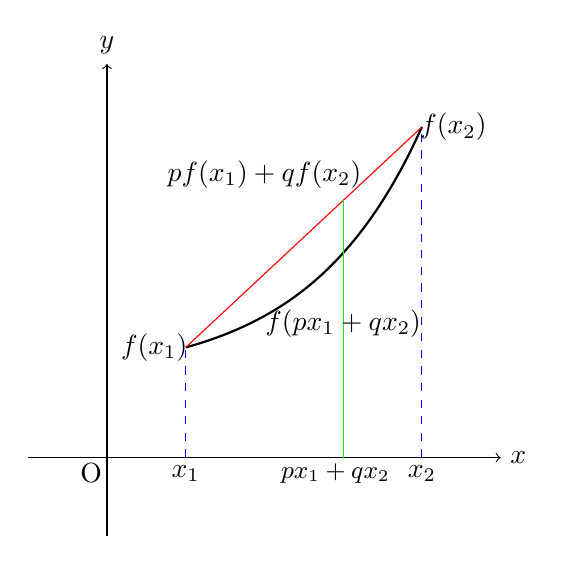
\begin{tikzpicture}
		\draw[->] (-1,0) -- (5,0) node[right] {$x$};
		\draw[->] (0,-1) -- (0,5) node[above] {$y$};
		\draw[thick, domain=1:4, smooth, variable=\x] plot ({\x},{0.2*2^(\x)+1});
		\draw[red] (1,1.4) -- (4,4.2);
		\draw[green] (3,0) -- (3,3.27);
		\draw[dashed,blue] (1,0) -- (1,1.4);
		\draw[dashed,blue] (4,0) -- (4,4.2);
		\node at (1,-0.2) {$x_{1}$};
		\node at (4,-0.2) {$x_{2}$};
		\node at (2.9,-0.2) {\small{$px_{1}+qx_{2}$}};
		\node at (0.6,1.4) {$f(x_{1})$};
		\node at (4.4,4.2) {$f(x_{2})$};
		\node at (3,1.7) {$f(px_{1}+qx_{2})$};
		\node at (2,3.6) {$pf(x_{1})+qf(x_{2})$};
		\node at (-0.2,-0.2) {O};
	\end{tikzpicture}
	\caption{凹函数性质}
	\label{Figure: 凹函数性质}
\end{figure}
\myspace{1}
\begin{solution}
	\begin{anymark}[凹函数性质]
		我们不妨假设$f(x)$在$(a,b)$上是凹函数,我们有以下的定理.
		
		$$\forall x_{1},x_{2},\cdots,x_{n}\in(a,b), x_{1}<x_{2}<\cdots<x_{n}, \exists p_{1},p_{2},\cdots,p_{n}>0,\sum\limits_{i=1}^{n}p_{n}=1,\ s.t. \sum\limits_{i=1}^{n}p_{i}f(x_{i})\geq f(\sum\limits_{i=1}^{n}p_{i}x_{i})$$
		\begin{proof}
			
			(1). 当$n=1$时,原命题显然成立.
			
			(2). 当$n=2$时,原命题等价于: 
			$$p+q=1,\ f(px_{1}+qx_{2})\leq pf(x_{1})+qf(x_{2})$$
			
			我们由 $Figure: $\ref{Figure: 凹函数性质}得到: 
			$$\left\lbrace
			\begin{array}{l}
				px_{1}+qx_{2}>(p+q)x_{1}=x_{1}\\
				px_{1}+qx_{2}<(p+q)x_{2}=x_{2}
			\end{array}
			\right. px_{1}+qx_{2}\in(x_{1},x_{2})$$
			
			$$\dfrac{l-f(x_{1})}{f(x_{2})-f(x_{1})}=\dfrac{px_{1}+qx_{2}-x_{1}}{x_{2}-x_{1}}=q\Rightarrow l=qf(x_{1})+(1-q)f(x_{1})=pf(x_{1})+qf(x_{2})$$
			
			(3). 假设当$n=k$时,我们有: $$\sum\limits_{i=1}^{k}p_{i}f(x_{i})\geq f(\sum\limits_{i=1}^{k}p_{i}x_{i})$$
			
			当$n=k+1$时,我们有: 
			\begin{eqnarray*}
				f(x_{1}+x_{2}+\cdots+x_{k}+x_{k+1})&=&f((1-x_{k+1})[\frac{x_{1}}{1-p_{k+1}}+\frac{x_{2}}{1-p_{k+1}}+\cdots+\frac{x_{k}}{1-p_{k+1}}+p_{k+1}x_{k+1}])\\
				&\leq& p_{k+1}f(x_{k+1})+\dfrac{1}{1-p_{k+1}}f(\sum\limits_{i=1}^{k}\dfrac{p_{i}}{1-p_{k+1}}x_{i})\\
				&\leq & \sum\limits_{i=1}^{k+1}p_{i}f(x_{i})
			\end{eqnarray*}
		\end{proof}
	\end{anymark}
	原命题等价于: 
	$$\lim\limits_{n\rightarrow+\infty}e^{\sum\limits_{i=1}^{n}f(\frac{i}{n})\frac{i}{n}}\leq \lim\limits_{n\rightarrow+\infty}\sum\limits_{i=1}^{n}\frac{1}{n}e^{f(\frac{i}{n})}$$
	
	我们得到: 
	$$e^{\int_{0}^{1}f(x)dx}\leq \int_{0}^{1}e^{f(x)}dx$$
\end{solution}
\myspace{1}

\hl{\textbf{\textit{June 30}}}

1. 求极限$\lim\limits_{x\rightarrow 0}\int_{0}^{x}(\dfrac{\arctan t}{t})^{\dfrac{1}{\int_{0}^{t}\ln(1+u)du}}\cot xdt$
\myspace{1}
\begin{solution}
	
	原极限等价于: 
	\begin{eqnarray*}
		I&=&\lim\limits_{x\rightarrow 0}\dfrac{\cos x\int_{0}^{x}(\dfrac{\arctan t}{t})^{\dfrac{1}{\int_{0}^{t}\ln(1+u)du}}}{\sin x}\\
		&=&\lim\limits_{x\rightarrow 0}\dfrac{\int_{0}^{x}(\dfrac{\arctan t}{t})^{\dfrac{1}{\int_{0}^{t}\ln(1+u)du}}dt}{x}\\
		&=&e^{\lim\limits_{x\rightarrow 0}\dfrac{\ln(\frac{\arctan x}{x})}{\int_{0}^{x}\ln(1+u)du}}\\
		&=&e^{\lim\limits_{x\rightarrow 0}\dfrac{-\frac{2}{3}x^2}{\int_{0}^{x}\ln(1+u)du}}\\
		&=&e^{-\frac{2}{3}}
	\end{eqnarray*}
\end{solution}
\myspace{1}

2. $f(x)$在$[0,1]$上连续,我们有$\int_{0}^{1}xf(x)dx=1,\ \int_{0}^{1}f(x)dx=0$,证明: $$\exists\xi\in(0,1),\ s.t. |f(\xi)|\geq 4$$
\myspace{1}
\begin{solution}
	
	我们由$\int_{0}^{1}xf(x)dx=1,\ \int_{0}^{1}f(x)dx=0$得到: 
	$$\int_{0}^{1}(x+a)f(x)=1\Rightarrow \int_{0}^{1}|x+a||f(x)|\geq 1$$
	
	我们假设$f(x)<4$,我们得到: 
	$$4\int_{0}^{1}|x+a|dx>1$$
	
	我们有: $$4\int_{0}^{1}|x+a|dx=\left\lbrace
	\begin{array}{l}
		4a+2,a\geq 0\\
		-4a-2,a\leq -1\\
		4a^2+4a+2,a\in(-1,0)
	\end{array}
	\right. $$
	
	我们要得出矛盾,即令$4\int_{0}^{1}|x+a|dx\leq 1$,我们令$a=-\dfrac{1}{2}$,$4\int_{0}^{1}|x+a|dx=1$矛盾!!!
	
	综上所述,我们得到: $\exists\xi\in(0,1),\ s.t. |f(\xi)|\geq 4$
\end{solution}
\myspace{1}